\documentclass{article}
\usepackage{fancyhdr}
\usepackage{geometry}
\usepackage{amsmath}
\usepackage{amssymb}
\usepackage{tikz}  % Add this package

\geometry{
    a4paper,
    top=2cm,
    bottom=2cm,
    left=2.5cm,
    right=2.5cm
}

\pagestyle{fancy}
\fancyhf{}
\rhead{Patrick Brown}
\lhead{Optimization}
\cfoot{\thepage}

\begin{document}

\begin{center}
    \Large\textbf{The University of Texas at Austin}\\
    \Large\textbf{Optimization}\\
    \large Homework 2\\
    \normalsize Patrick Brown
\end{center}

\noindent\textbf{Instructors:} Constantine Caramanis, Sujay Sanghavi\\
\textbf{Keywords:} Linear Programming, Graphical Solutions, LP Formulation
\vspace{1cm}

\noindent Please submit your solutions as a single pdf file. If you have code or figures, please include these in the pdf.

\vspace{1cm}

\section*{Problem 1}

Let's solve the problem step by step by formulating an explicit linear program (LP) that models the given scenario. We'll define the decision variables, construct the objective function, and formulate the constraints in matrix form.

\subsection*{1. Decision Variables}

Let $x_{ij}$ represent the number of units of Widget $j$ produced by Worker $i$, where:

\begin{itemize}
    \item $i = 1, 2, 3, 4$ (workers)
    \item $j = A, B, C$ (widgets)
\end{itemize}

So, we have 12 decision variables:

\begin{align*}
    & x_{1A},\ x_{1B},\ x_{1C} \\
    & x_{2A},\ x_{2B},\ x_{2C} \\
    & x_{3A},\ x_{3B},\ x_{3C} \\
    & x_{4A},\ x_{4B},\ x_{4C}
\end{align*}

\subsection*{2. Objective Function}

We aim to minimize the total cost of production. The total cost is calculated based on the time each worker spends on each widget and their respective hourly rates.

\textbf{Cost Calculation:}

\begin{itemize}
    \item \textbf{Time per unit (in minutes):} $t_{ij}$
    \item \textbf{Cost per hour for Worker $i$ on Widget $j$:} $c_{ij}$
\end{itemize}

The total cost for Worker $i$ on Widget $j$ is:

\[ \text{Cost}_{ij} = \left( \frac{t_{ij} \times x_{ij}}{60} \right) \times c_{ij} \]

Therefore, the objective function to minimize is:

\begin{align*}
    \text{Minimize } Z = & \frac{1}{60} (8x_{1A} \cdot 20 + 10x_{1B} \cdot 20 + 13x_{1C} \cdot 20 \\
    & + 7x_{2A} \cdot 22 + 12x_{2B} \cdot 22 + 14x_{2C} \cdot 22 \\
    & + 4x_{3A} \cdot 25 + 8x_{3B} \cdot 25 + 9x_{3C} \cdot 25 \\
    & + 10x_{4A} \cdot 18 + 15x_{4B} \cdot 18 + 17x_{4C} \cdot 18)
\end{align*}

\subsection*{3. Constraints}

\begin{enumerate}
    \item \textbf{Time Constraints:}
    \begin{itemize}
        \item Worker 1: $8x_{1A} + 10x_{1B} + 13x_{1C} \leq 2100$
        \item Worker 2: $7x_{2A} + 12x_{2B} + 14x_{2C} \leq 2100$
        \item Worker 3: $4x_{3A} + 8x_{3B} + 9x_{3C} \leq 2100$
        \item Worker 4: $10x_{4A} + 15x_{4B} + 17x_{4C} \leq 2100$
    \end{itemize}

    \item \textbf{Demand Constraints:}
    \begin{itemize}
        \item Widget A: $x_{1A} + x_{2A} + x_{3A} + x_{4A} \geq 100$
        \item Widget B: $x_{1B} + x_{2B} + x_{3B} + x_{4B} \geq 150$
        \item Widget C: $x_{1C} + x_{2C} + x_{3C} + x_{4C} \geq 100$
    \end{itemize}

    \item \textbf{Non-negativity Constraints:}
    \[ x_{ij} \geq 0 \quad \text{for all } i, j \]
\end{enumerate}

\subsection*{4. Interpretation}

By solving this linear program, the company will determine the optimal assignment of workers to widget production tasks that meets the demand at the minimum possible cost, considering the workers' efficiency and wage rates for different widgets.

\subsection*{Note}

\begin{itemize}
    \item The time is converted to minutes to maintain consistency.
    \item Costs are calculated on an hourly basis, so we divide the total minutes by 60 to convert to hours.
    \item The demand constraints are represented as inequalities (greater than or equal to) to ensure minimum production requirements are met.
\end{itemize}

\section*{Problem 2}
\begin{enumerate}
    \item Consider the following LP:
    \begin{align*}
        \min : & \quad -x_1 - x_2 \\
        \text{s.t. : } & \quad x_1 + 3x_2 \leq 3 \\
        & \quad 2x_1 + x_2 \leq 3 \\
        & \quad 4x_1 + 4x_2 \geq 1 \\
        & \quad x_1, x_2 \geq 0.
    \end{align*}
    \begin{enumerate}
        \item Draw the feasible set.
        \item Compute explicitly all extreme points. Which is the optimal one?
        \item Now use the level set method to find the optimal solution. That is, draw the level sets of the objective function, and show that you find the same optimal solution as you did by enumeration in the previous part of this exercise.
    \end{enumerate}
\end{enumerate}

\section*{Solution}

\subsection*{Part (a): Draw the Feasible Set}

\textbf{Step 1:} Interpret the Constraints
\begin{itemize}
\item \textbf{Constraint (1):} $x_1 + 3x_2 \leq 3$
\item \textbf{Constraint (2):} $2x_1 + x_2 \leq 3$
\item \textbf{Constraint (3):} $4x_1 + 4x_2 \geq 1$
\item \textbf{Non-negativity Constraints (4):} $x_1 \geq 0, \ x_2 \geq 0$
\end{itemize}

\textbf{Step 2:} Simplify Constraint (3)

Divide both sides by 4:
\[x_1 + x_2 \geq 0.25\]

\textbf{Step 3:} Plot the Constraints

\textbf{Step 4:} Identify the Feasible Region

The feasible region is the convex polygon defined by the intersection of these constraints, bounded within the first quadrant.

\begin{figure}[h]
\centering
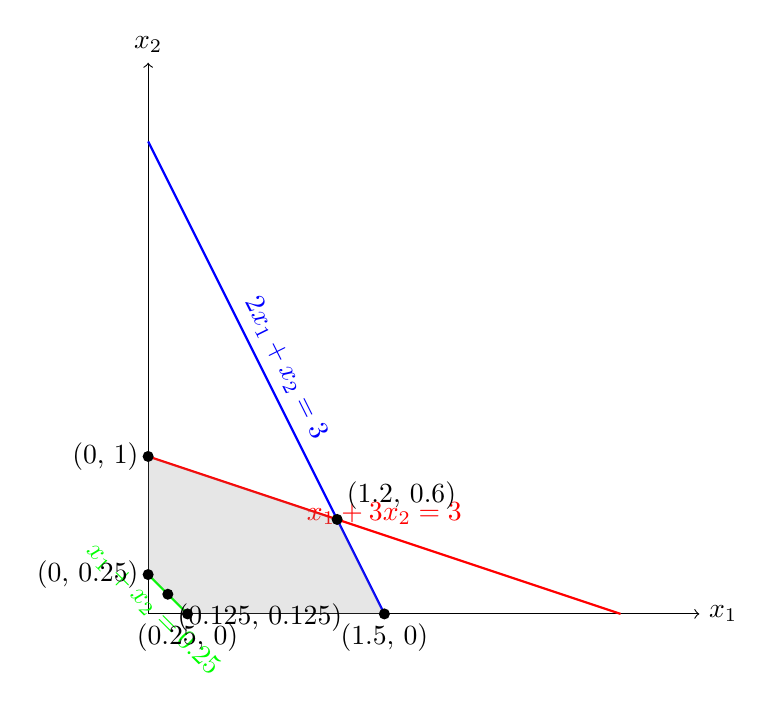
\begin{tikzpicture}[scale=2]
    % Axes
    \draw[->] (0,0) -- (3.5,0) node[right] {$x_1$};
    \draw[->] (0,0) -- (0,3.5) node[above] {$x_2$};
    
    % Constraints
    \draw[red, thick] (0,1) -- (3,0) node[midway, above] {$x_1 + 3x_2 = 3$};
    \draw[blue, thick] (0,3) -- (1.5,0) node[midway, above, sloped] {$2x_1 + x_2 = 3$};
    \draw[green, thick] (0.25,0) -- (0,0.25) node[midway, below, sloped] {$x_1 + x_2 = 0.25$};
    
    % Feasible region
    \fill[gray, opacity=0.2] (0.25,0) -- (1.5,0) -- (1.2,0.6) -- (0,1) -- (0,0.25) -- cycle;
    
    % Points of interest
    \fill (1.2,0.6) circle (1pt) node[above right] {(1.2, 0.6)};
    \fill (0,1) circle (1pt) node[left] {(0, 1)};
    \fill (1.5,0) circle (1pt) node[below] {(1.5, 0)};
    \fill (0,0.25) circle (1pt) node[left] {(0, 0.25)};
    \fill (0.25,0) circle (1pt) node[below] {(0.25, 0)};
    \fill (0.125,0.125) circle (1pt) node[below right] {(0.125, 0.125)};
\end{tikzpicture}
\caption{Feasible region for the linear program}
\label{fig:feasible_region}
\end{figure}

The feasible region is the shaded area in Figure \ref{fig:feasible_region}, which is the convex polygon defined by the intersection of these constraints, bounded within the first quadrant.

\subsection*{Part (b): Find All Extreme Points}

All extreme points are:
\begin{itemize}
\item $(1.2, 0.6)$
\item $(0, 1)$
\item $(1.5, 0)$
\item $(0, 0.25)$
\item $(0.25, 0)$
\item $(0.125, 0.125)$
\end{itemize}

The optimal extreme point is $(1.2, 0.6)$ with an objective value of $-1.8$.

\subsection*{Part (c): Use the Level Set Method}

\textbf{Step 1:} Write the objective function as a level set
\[x_1 + x_2 = k\]

\textbf{Step 2:} Plot level lines for increasing values of $k$:
\begin{itemize}
\item $x_1 + x_2 = 0.25$
\item $x_1 + x_2 = 0.5$
\item $x_1 + x_2 = 1$
\item $x_1 + x_2 = 1.5$
\item $x_1 + x_2 = 1.8$
\end{itemize}

\textbf{Step 3:} Move Level Lines to Find the Optimal Point

Slide the line $x_1 + x_2 = k$ upwards (increasing $k$) while it still intersects the feasible region.

\textbf{Step 4:} Identify the Optimal Solution
\begin{itemize}
\item The highest value of $k$ that intersects the feasible region is $1.8$.
\item This occurs at the point $(x_1, x_2) = (1.2, 0.6)$.
\end{itemize}

\section*{Conclusion}

\textbf{(a)} The feasible set is the convex polygon defined by the intersection of the constraints, bounded within the first quadrant.

\textbf{(b)} The optimal extreme point is $(1.2, 0.6)$ with an objective value of $-1.8$.

\textbf{(c)} By using the level set method and moving the line $x_1 + x_2 = k$ to the highest possible value within the feasible region, we find the optimal solution at $(1.2, 0.6)$, confirming our previous result.

\section*{Problem 3}

\begin{enumerate}
    \item minimize $\|Ax - b\|_1$ subject to $\|x\|_\infty \leq 1$.
    \item minimize $\|x\|_1$ subject to $\|Ax - b\|_\infty \leq 1$.
    \item minimize $\|Ax - b\|_1 + \|x\|_\infty$.
\end{enumerate}

In each problem, $A \in \mathbb{R}^{m\times n}$ and $b \in \mathbb{R}^m$ are given, and $x \in \mathbb{R}^n$ is the optimization variable.
As a reminder, the 1-norm and infinity norm of $x \in \mathbb{R}^n$ are defined as

\begin{align*}
    \|x\|_1 &= \sum_{i=1}^n |x_i|, \\
    \|x\|_\infty &= \max_{i=1,\ldots,n} |x_i|
\end{align*}

\subsection*{Solution}

All three problems can be transformed into linear programs by introducing auxiliary variables to handle the absolute values and maximum functions.

\subsubsection*{Problem A}

Minimize $\|Ax - b\|_1$ subject to $\|x\|_\infty \leq 1$

\textbf{Step 1:} Introduce auxiliary variables $t_i \geq 0$ such that:
\begin{align*}
    t_i \geq (Ax - b)_i \quad \text{and} \quad t_i \geq -(Ax - b)_i \quad \text{for } i = 1, \dots, m
\end{align*}

\textbf{Step 2:} Rewrite the constraint $\|x\|_\infty \leq 1$ as:
\begin{align*}
    -1 \leq x_j \leq 1 \quad \text{for } j = 1, \dots, n
\end{align*}

\textbf{Step 3:} The linear program becomes:
\begin{align*}
    \text{Minimize} \quad & \sum_{i=1}^m t_i \\
    \text{Subject to} \quad & t_i \geq (Ax - b)_i, \quad i = 1, \dots, m \\
    & t_i \geq -(Ax - b)_i, \quad i = 1, \dots, m \\
    & -1 \leq x_j \leq 1, \quad j = 1, \dots, n \\
    & t_i \geq 0, \quad i = 1, \dots, m
\end{align*}

\subsubsection*{Problem B}

Minimize $\|x\|_1$ subject to $\|Ax - b\|_\infty \leq 1$

\textbf{Step 1:} Introduce auxiliary variables $t_j \geq 0$ such that:
\begin{align*}
    t_j \geq x_j \quad \text{and} \quad t_j \geq -x_j \quad \text{for } j = 1, \dots, n
\end{align*}

\textbf{Step 2:} Rewrite the constraint $\|Ax - b\|_\infty \leq 1$ as:
\begin{align*}
    -1 \leq (Ax - b)_i \leq 1 \quad \text{for } i = 1, \dots, m
\end{align*}

\textbf{Step 3:} The linear program becomes:
\begin{align*}
    \text{Minimize} \quad & \sum_{j=1}^n t_j \\
    \text{Subject to} \quad & t_j \geq x_j, \quad j = 1, \dots, n \\
    & t_j \geq -x_j, \quad j = 1, \dots, n \\
    & -1 \leq (Ax - b)_i \leq 1, \quad i = 1, \dots, m \\
    & t_j \geq 0, \quad j = 1, \dots, n
\end{align*}

\subsubsection*{Problem C}

Minimize $\|Ax - b\|_1 + \|x\|_\infty$

\textbf{Step 1:} Introduce auxiliary variables $t_i \geq 0$ for $\|Ax - b\|_1$ such that:
\begin{align*}
    t_i \geq (Ax - b)_i \quad \text{and} \quad t_i \geq -(Ax - b)_i \quad \text{for } i = 1, \dots, m
\end{align*}

\textbf{Step 2:} Introduce an auxiliary variable $s \geq 0$ for $\|x\|_\infty$ such that:
\begin{align*}
    s \geq x_j \quad \text{and} \quad s \geq -x_j \quad \text{for } j = 1, \dots, n
\end{align*}

\textbf{Step 3:} The linear program becomes:
\begin{align*}
    \text{Minimize} \quad & \sum_{i=1}^m t_i + s \\
    \text{Subject to} \quad & t_i \geq (Ax - b)_i, \quad i = 1, \dots, m \\
    & t_i \geq -(Ax - b)_i, \quad i = 1, \dots, m \\
    & s \geq x_j, \quad j = 1, \dots, n \\
    & s \geq -x_j, \quad j = 1, \dots, n \\
    & t_i \geq 0, \quad i = 1, \dots, m \\
    & s \geq 0
\end{align*}

All three problems have been transformed into linear programs that can be efficiently solved using standard optimization software.

\section*{Problem 4}

Formulate the following problems as LPs.

\subsection*{(a)}

Given $A \in \mathbb{R}^{m\times n}, b \in \mathbb{R}^m$, minimize

\[
\sum_{i=1}^m \max\{0, a_i^T x + b_i\}
\]

The variable is $x \in \mathbb{R}^n$.

\textbf{Solution:}

To formulate this problem as a linear program (LP), we introduce auxiliary variables $s_i \geq 0$ to represent each max term.

\textbf{Variables:}
\begin{itemize}
    \item $x \in \mathbb{R}^n$
    \item $s \in \mathbb{R}^m$
\end{itemize}

\textbf{Objective Function:}
\[
\min_{x,\,s} \quad \sum_{i=1}^m s_i
\]

\textbf{Constraints:}
\begin{align*}
s_i &\geq a_i^T x + b_i, \quad i = 1, \ldots, m \\
s_i &\geq 0, \quad i = 1, \ldots, m
\end{align*}

\textbf{Complete LP Formulation:}
\begin{align*}
\min_{x,\,s} \quad & \sum_{i=1}^m s_i \\
\text{subject to} \quad & s_i \geq a_i^T x + b_i, \quad i = 1, \ldots, m \\
& s_i \geq 0, \quad i = 1, \ldots, m \\
& x \in \mathbb{R}^n \\
& s \in \mathbb{R}^m
\end{align*}

This LP can now be solved using standard linear programming techniques. The auxiliary variables $s_i$ effectively capture the positive part of $a_i^T x + b_i$, ensuring that $s_i = \max\{0, a_i^T x + b_i\}$ in the optimal solution.


\section*{Problem 6}

For each of the following LPs, express the optimal value and the optimal solution in terms of the problem parameters $(c, k, d, \alpha, d_1, d_2, \ldots)$. If the optimal solution is not unique, it is sufficient to give one optimal solution.

\begin{enumerate}
    \item[(a)] 
    \begin{align*}
        \text{minimize} \quad & c^T x \\
        \text{subject to} \quad & 0 \leq x \leq 1
    \end{align*}
    The variable is $x \in \mathbb{R}^n$.

    \textbf{Solution:}

    \textbf{Optimal Solution $x^*$:}
    \[
    x_i^* = \begin{cases}
    1 & \text{if } c_i \leq 0, \\
    0 & \text{if } c_i > 0.
    \end{cases}
    \]

    \textbf{Optimal Value $v^*$:}
    \[
    v^* = \sum_{i=1}^{n} \min(0, c_i) = \sum_{i: c_i \leq 0} c_i.
    \]

    \textbf{Explanation:}
    \begin{itemize}
    \item For each component $x_i$, we minimize $c_i x_i$ over $x_i \in [0,1]$.
    \item If $c_i > 0$, setting $x_i = 0$ minimizes $c_i x_i$.
    \item If $c_i \leq 0$, setting $x_i = 1$ minimizes $c_i x_i$.
    \end{itemize}

    \item[(b)]
    \begin{align*}
        \text{minimize} \quad & c^T x \\
        \text{subject to} \quad & -1 \leq x \leq 1
    \end{align*}
    The variable is $x \in \mathbb{R}^n$.

    \textbf{Solution:}

    \textbf{Optimal Solution $x^*$:}
    \[
    x_i^* = \begin{cases}
    -1 & \text{if } c_i \geq 0, \\
    1 & \text{if } c_i \leq 0.
    \end{cases}
    \]

    \textbf{Optimal Value $v^*$:}
    \[
    v^* = \sum_{i: c_i \geq 0} (-c_i) + \sum_{i: c_i \leq 0} c_i = -\sum_{i: c_i \geq 0} c_i + \sum_{i: c_i \leq 0} c_i.
    \]

    \textbf{Explanation:}
    \begin{itemize}
    \item For each $x_i$, we minimize $c_i x_i$ over $x_i \in [-1,1]$.
    \item If $c_i \geq 0$, setting $x_i = -1$ minimizes $c_i x_i$.
    \item If $c_i \leq 0$, setting $x_i = 1$ minimizes $c_i x_i$.
    \end{itemize}

    \item[(c)]
    \begin{align*}
        \text{minimize} \quad & c^T x \\
        \text{subject to} \quad & -1 \leq 1^T x \leq 1
    \end{align*}
    The variable is $x \in \mathbb{R}^n$.

    \textbf{Solution:}

    \textbf{Optimal Value $v^*$:}
    \begin{itemize}
        \item If $c \neq 0$:
        \[
        v^* = -\infty \quad \text{(The LP is unbounded below)}
        \]
        \item If $c = 0$:
        \[
        v^* = 0
        \]
    \end{itemize}

    \textbf{Optimal Solution $x^*$:}
    \begin{itemize}
        \item If $c \neq 0$: No finite optimal solution exists since the LP is unbounded below.
        \item If $c = 0$: Any $x$ satisfying $-1 \leq 1^T x \leq 1$.
    \end{itemize}

    \textbf{Explanation:}
    \begin{itemize}
    \item The LP is unbounded below unless $c = 0$.
    \item For $c \neq 0$, one can make $c^T x$ arbitrarily negative while satisfying the constraint.
    \item If $c = 0$, $c^T x = 0$ for all feasible $x$.
    \end{itemize}

    \item[(d)]
    \begin{align*}
        \text{minimize} \quad & c^T x \\
        \text{subject to} \quad & 1^T x = 1, \quad x \geq 0
    \end{align*}
    The variable is $x \in \mathbb{R}^n$.

    \textbf{Solution:}

    \textbf{Optimal Solution $x^*$:}

    Let $i^* \in \arg\min_{i} c_i$. Then,
    \[
    x_i^* = \begin{cases}
    1 & \text{if } i = i^*, \\
    0 & \text{otherwise}.
    \end{cases}
    \]

    \textbf{Optimal Value $v^*$:}
    \[
    v^* = c_{i^*} = \min_{i} c_i.
    \]

    \textbf{Explanation:}
    \begin{itemize}
    \item The feasible region is the simplex, and the minimum of a linear function over a simplex occurs at a vertex.
    \item Choosing the variable with the smallest $c_i$ minimizes $c^T x$.
    \end{itemize}

    \item[(e)]
    \begin{align*}
        \text{maximize} \quad & c^T x \\
        \text{subject to} \quad & 1^T x = k, \quad 0 \leq x \leq 1
    \end{align*}
    The variable is $x \in \mathbb{R}^n$. $k$ is an integer with $1 \leq k \leq n$.

    \textbf{Solution:}

    \textbf{Optimal Solution $x^*$:}

    Let $c_{(1)} \geq c_{(2)} \geq \dots \geq c_{(n)}$ be the sorted components of $c$. Then,
    \[
    x_i^* = \begin{cases}
    1 & \text{for } i = 1, 2, \dots, k, \\
    0 & \text{otherwise}.
    \end{cases}
    \]

    \textbf{Optimal Value $v^*$:}
    \[
    v^* = \sum_{i=1}^{k} c_{(i)}.
    \]

    \textbf{Explanation:}
    \begin{itemize}
    \item We aim to maximize $c^T x$ by selecting $k$ variables to set to 1 (since $x_i \leq 1$) and the rest to 0.
    \item Choosing the $k$ largest $c_i$ values ensures the maximum $c^T x$.
    \end{itemize}
\end{enumerate}

\textbf{Note:} In all problems, since the objective function is linear and the feasible region is convex, the optimal solution occurs at an extreme point of the feasible region.

\end{document}
